%!TEX root = ../thesis.tex

\section{Convolutional Neural Network (CNN)}

  本研究の学習器は畳み込みニューラルネットワーク(Convolutional Neural Network:CNN)で,これは画像認識などで用いられている\cite{yann1}\cite{alex}.畳み込み層とプーリング層を含む構造で,多次元配列の形式データを効率的に処理するように設計されている.例として,LeCunら\cite{yann1}は,畳み込み層とプーリング層を連続して接続するネットワークを用いることで,手書き文字を識別できることを示した(\figref{Fig:yann_CNN}).また,Krizhevskyら\cite{alex}は,深い畳み込みニューラルネットワークを用いることで,1000種類のクラスに分類できることを示し(\figref{Fig:deep_convolutional_neural_networks}),ILSVRC(ImageNet Large Scale Visual Recognition Challenge)2012で優勝した.

  CNNは,主に畳み込み層,プーリング層,および全結合層から構成される.以下に,それぞれの特徴を記す.

  \begin{enumerate}
    \item 畳み込み層\\
    入力データに対してフィルターを適用し,特徴を抽出した特徴マップを出力する層
    \item プーリング層\\
    特徴マップのサイズを削減し,特徴の位置に対する頑健性を向上させるために,領域内の最大値や平均値を取る操作を行う層
    \item 全結合層\\
    畳み込み層とプーリング層で抽出された特徴を組み合わせて,最終的な出力を生成する層
  \end{enumerate}

  \begin{figure}[h]
    \centering
    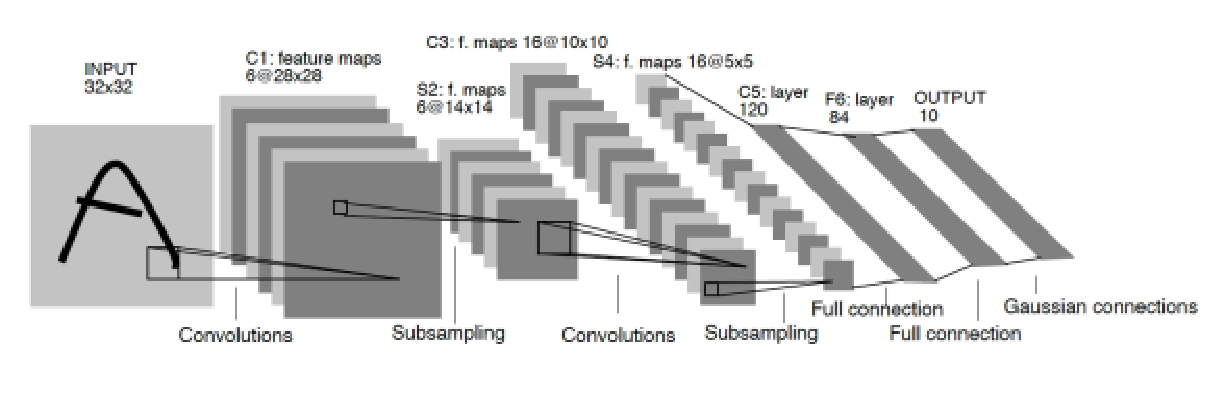
\includegraphics[keepaspectratio, scale=0.50] {images/eps/yann_CNN}
    \caption[Training the neural network]{Training the neural network (source: \cite{yann1})}
    \label{Fig:yann_CNN}
  \end{figure}

\newpage

  \begin{figure}[h]
    \centering
    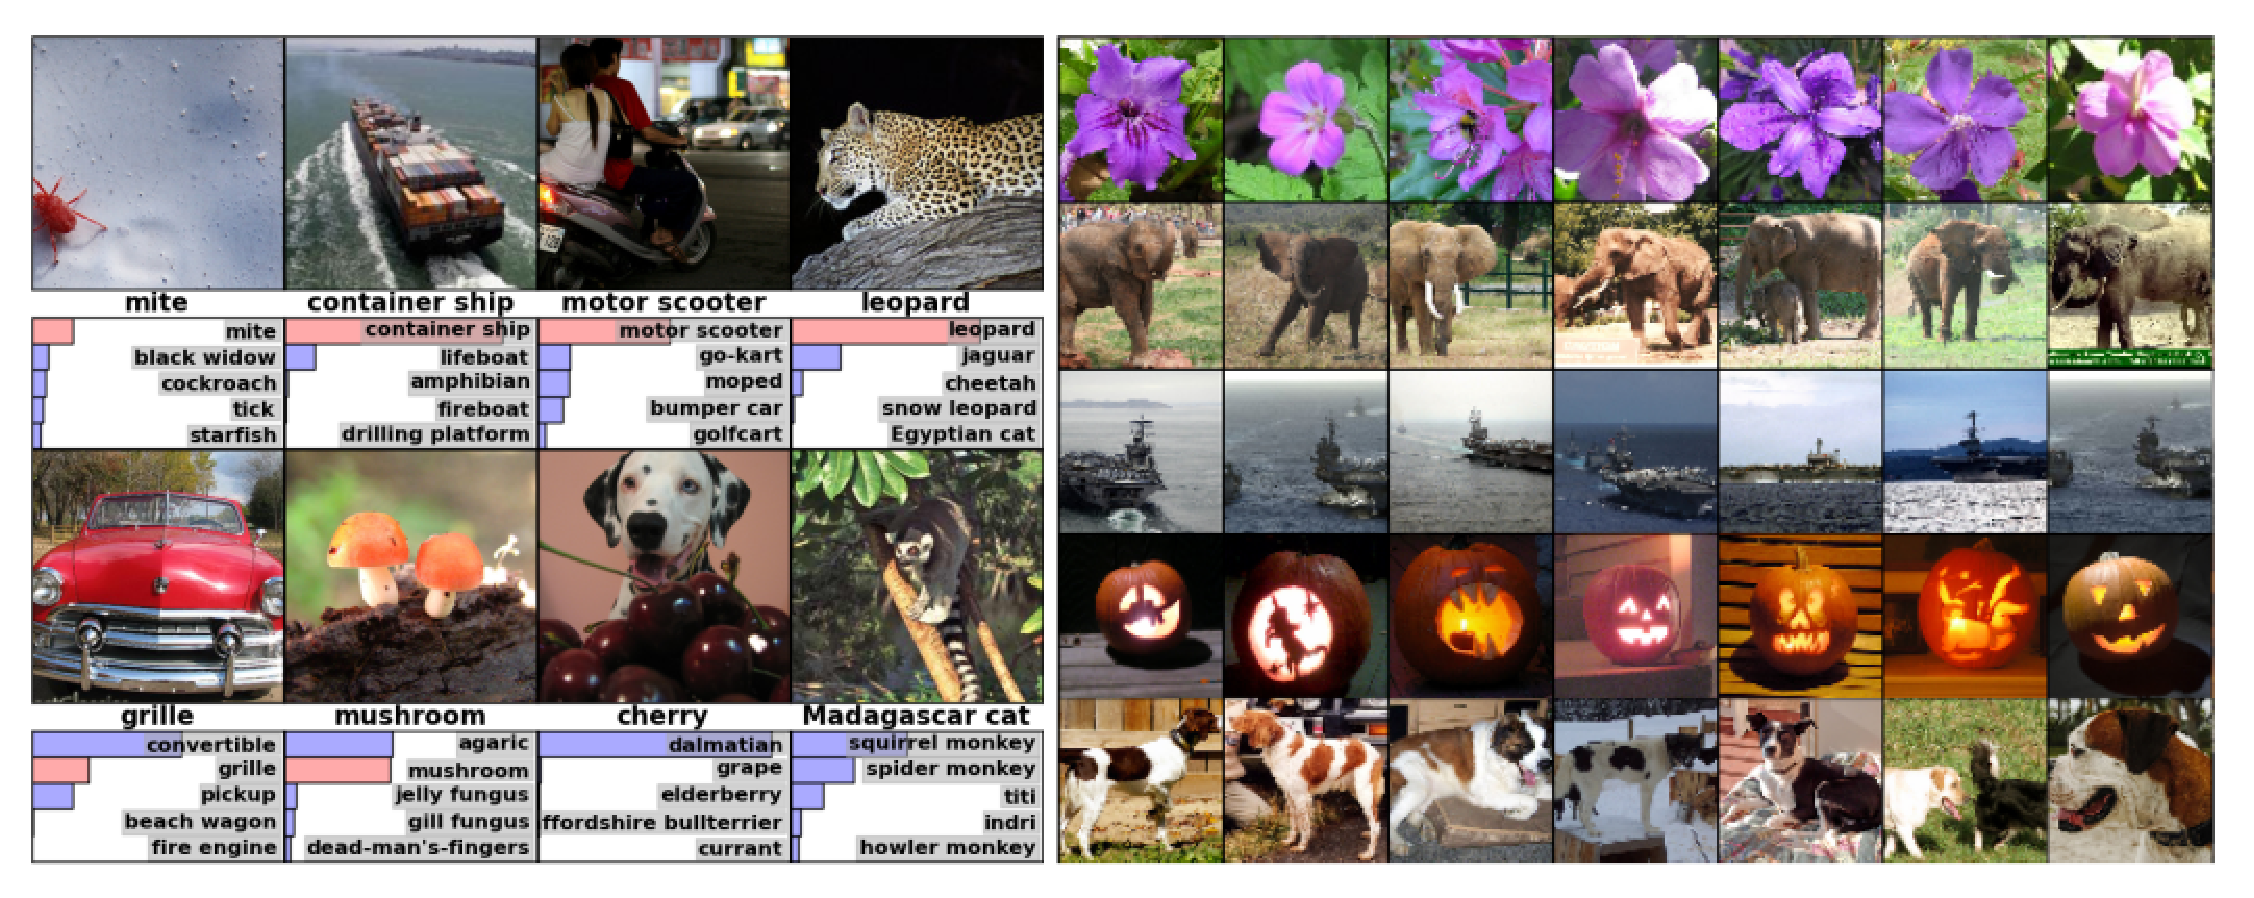
\includegraphics[keepaspectratio, scale=0.30] {images/eps/deep_convolutional_neural_networks}
    \caption[ImageNet classification with deep convolutional neural network]{ImageNet classification with deep convolutional neural network (source: \cite{alex})}
    \label{Fig:deep_convolutional_neural_networks}
  \end{figure}


\newpage
